\subsection*{\comp.hdl}
\begin{flushleft}
	Figure \ref{fig:complex_mixer} diagrams the complex mixer.\medskip

	\begin{figure}[h]
		\centering\captionsetup{type=figure}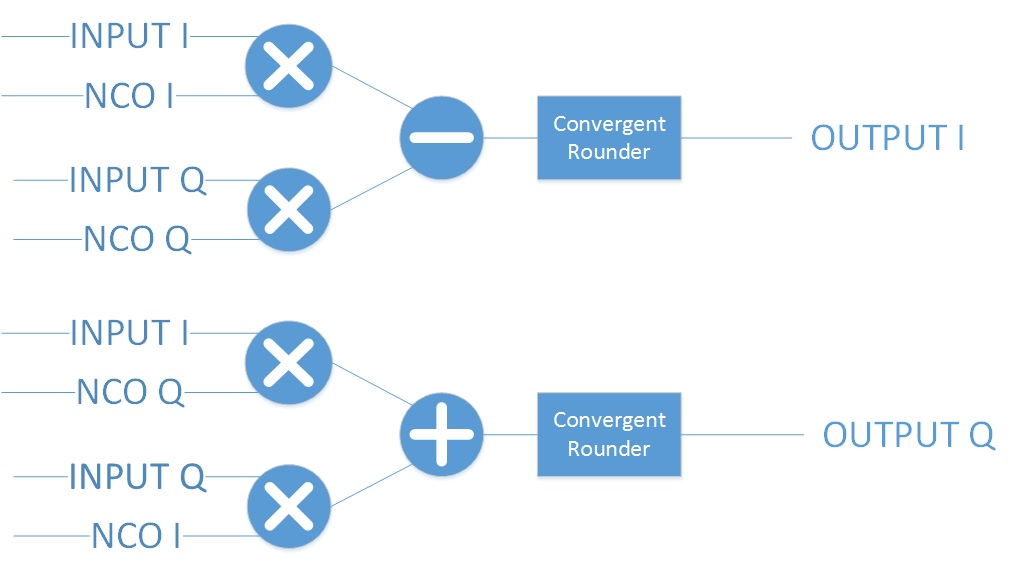
\includegraphics[scale=0.4]{complex_mixer_block_diagram}
		\captionof{figure}{Complex Mixer Functional Diagram}
		\label{fig:complex_mixer}
	\end{figure}
	Build time parameters can be used to control the width of the NCO data output, the width of the input data, and the number of stages in the Coordinate Rotation Digital Computer (CORDIC) used to implement the NCO. Additionally, there is a parameter to control insertion of a peak detection circuit.\medskip

	An \verb+enable+ input is available to either enable (true) or bypass (false) the circuit. In bypass mode, pipe-lining registers are not used. FPGA multipliers are used to process input data at the full clock rate. This worker will produce valid output two clock cycles after each valid input.
\end{flushleft}
